\documentclass[11.7pt]{llncs}
\usepackage{llncsdoc}
\usepackage[hidelinks]{hyperref}
\usepackage{listings}
\usepackage{tabularx}
\usepackage{ltablex}
\usepackage{graphicx}
\usepackage{minted}
\setcounter{secnumdepth}{4}
\setcounter{tocdepth}{4}
\usepackage{float}
\restylefloat{figure}
\usepackage{indentfirst}
\usepackage  {acronym}
\usepackage{hyperref}
\usepackage{array}
\newcolumntype{Y}{>{\centering\arraybackslash}X}
\usepackage{listings}
\usepackage[hidelinks]{hyperref}
\usepackage{graphicx}
\usepackage{color}
\usepackage{listings}
\usepackage{setspace}
\definecolor{Code}{rgb}{0,0,0}
\definecolor{Decorators}{rgb}{0.5,0.5,0.5}
\definecolor{Numbers}{rgb}{0.5,0,0}
\definecolor{MatchingBrackets}{rgb}{0.25,0.5,0.5}
\definecolor{Keywords}{rgb}{0,0,1}
\definecolor{self}{rgb}{0,0,0}
\definecolor{Strings}{rgb}{0,0.63,0}
\definecolor{Comments}{rgb}{0,0.63,1}
\definecolor{Backquotes}{rgb}{0,0,0}
\definecolor{Classname}{rgb}{0,0,0}
\definecolor{FunctionName}{rgb}{0,0,0}
\definecolor{Operators}{rgb}{0,0,0}
\definecolor{Background}{rgb}{0.98,0.98,0.98}
\lstdefinelanguage{Python}{
numbers=left,
numberstyle=\footnotesize,
numbersep=1em,
xleftmargin=1em,
framextopmargin=2em,
framexbottommargin=2em,
showspaces=false,
showtabs=false,
showstringspaces=false,
frame=l,
tabsize=4,
% Basic
basicstyle=\ttfamily\small\setstretch{1},
backgroundcolor=\color{Background},
% Comments
commentstyle=\color{Comments}\slshape,
% Strings
stringstyle=\color{Strings},
morecomment=[s][\color{Strings}]{"""}{"""},
morecomment=[s][\color{Strings}]{'''}{'''},
% keywords
morekeywords={len,import,from,class,def,for,while,if,is,in,elif,else,not,and,or,print,break,continue,return,True,False,None,access,as,,del,except,exec,finally,global,import,lambda,pass,print,raise,try,assert},
keywordstyle={\color{Keywords}\bfseries},
% additional keywords
morekeywords={[2]@invariant,pylab,numpy,np,scipy},
keywordstyle={[2]\color{Decorators}\slshape},
emph={self},
emphstyle={\color{self}\slshape},
%
}
\linespread{1.26}
%
\begin{document}


\begin{flushleft}
\thispagestyle{empty}
\centering { \LARGE \bf Malware Meta Crawler for MASS}
\vspace{34pt}

\centering \large
 MA-INF 3309 - Malware Analysis \\
 Lab Report\\
 
   Winter Semester 2016.17\\

		 University of Bonn\\


\vspace{46pt}
\centering \large
 Ehab Qadah\\
 
 \vspace{24pt}
 
 \today\\
 \rule{\textwidth}{1pt}
\end{flushleft}

\tableofcontents

\newpage
\begin{abstract}
On a daily basis, a huge number of new  software is discovered that performs different malicious activities. This makes the gathering of  malware samples from different parts of the Internet an important task for the IT security researchers, in oder to analyze them and develop defense mechanisms to avoid possible cyber attacks. The Malware Analysis and Storage System (MASS) aims to build a malware database to serve the security experts of the new submitted malware samples and offering the ability to store their analysis work results. In this report, we present a software tool is called  Malware Meta Crawler, which aims to automatically feed the MASS server's database of malware samples retrieved from different on-line sources and repositories. Furthermore, it enriches the information of the retrieved malware samples and creates semantic relations between them.
\end{abstract}


\begin{keywords}
malicious software, malware analysis, malware, worms, crawler, malware analysis and storage system (MASS)
\end{keywords}

\section{Introduction}

In the last decade, the usage of the Internet has increased and adopted in all sectors of business and industry as result of the digital
revolution. On the other hand, the wide usage of Internet creates a new opportunities for Cyber criminals to perform their malicious activities such as information theft and espionage.
Malicious Software  (malware) is any software that has a harmful intention and abuse the user's computer \cite{malware_analysis_def}. Malware is a common tool to perform cyber attacks that can be in different forms such as worm, virus, Trojan and spyware \cite{worms}.
According to Symantec, in 2015, 431 million  of new malware samples were discovered \cite{symantec}, which means over  one million per day. To protect  Internet users  the malware research community try hardly to study these malware samples, in order to build the counter measures and detect the new malware software or their malicious behavior, using different malware analysis techniques including static or dynamic analysis of malware samples \cite{malware_analysis}.

  
  \par In this work, we aim to develop Malware Meta Crawler system that feeds the  Malware Analysis and Storage System (MASS) \cite{mass} server's database with new malware samples retrieved from on-line sources and repositories that provide malicious domains, Uniform Resource Identifiers (URIs) \footnote{\url{https://tools.ietf.org/html/rfc3986}} and binaries. The retrieved samples are reported as connected  with malware activities or deliver malicious payload. Furthermore, the Malware Meta Crawler contains analysis units that analyze the malware samples to  enrich the samples with additional related data (e.g., IP of a malware domain). Furthermore, it detects the relations between the malware samples and submit them to the MASS server.
  \par To sum up, the goal of our system is to 
    build a comprehensive database of malicious softwares, to make the malware samples continuously available in one place, which helps the security researchers in their work.
  
  \par The remainder of this report is organized as follows.
  In Section~\ref{sec:sec2}, we present the related work and fundamental background . Section~\ref{sec:sec3} presents the general system overview. In Section~\ref{sec:sec4} we give the implementation details. Section~\ref{sec:sec5}
 provides the evaluation results. And finally, Section~\ref{sec:sec6} gives the overall conclusion and future work.
      
\section{Background and Related Work}
\label{sec:sec2}
 
In this section, we review some of the related work to our system and the required concepts that are used throughout the report. First, we provide an overview of the MASS eco-system. Then, we discuss the malware analysis techniques. Afterward, we provide a brief overview of related and similar systems. Finally, we present the used on-line sources of malware samples.


\subsection{Malware Analysis and Storage System (MASS)}

	The Malware Analysis and Storage System (MASS) serves as a platform for  providing malware samples and analysis results for security researchers\cite{mass}. All collected malware samples  and analysis results (reports) are stored in a database on the MASS server. The database of the MASS server contains malware samples submitted by malware researchers or retrieved by the malware meta crawler component. The MASS server is connected to several analysis systems which ease the process of sample reception and analysis. In addition to that MASS provides a web interface and REST APIs to access the malware samples and analysis results.
		
		\par The aim of MASS  is to provide a collaboration, scalable, open source  platform for malware analysis.
\subsection{MASS API Client}
The MASS API Client project provides a  programing API interface to the MASS server operations \cite{mass_api}, it is currently under the development phase. Nevertheless, we utilize the MASS API Client's functionalities to submit the malware samples to the MASS server and develop analysis systems to enrich the information of the submitted malware samples.


\subsection{Malware Analysis}
This section provides an overview of the malware analysis techniques (i.e., static and dynamic analysis).
Bayer, Ulrich, et al. \cite{malware_analysis_def} define the malware analysis as the process of identifying and understanding the capabilities and goals of a malicious software sample. 

\par In our system we analyze and process the malware samples to connect the related samples and enrich their information, this process is categorized as static analysis technique.

\subsubsection{Static Analysis}\hspace*{\fill} \\

\par The static analysis is a technique to analyze the malware sample by generating the corresponding assembly code to understand the control and data flow of the sample \cite{malware_analysis_def}, this method does not require to run the malware executable. 
\subsubsection{Dynamic Analysis}\hspace*{\fill} \\

While the dynamic analysis approach is to study the behavior of malware sample by executing it in isolated environment \cite{malware_analysis_def},  this technique requires to run the malware executable on a certain environment and find the effects of execution on the host system. 


\subsection{Sources of Malware Samples } 
\label{sec:sources}
This section presents the on-line sources that are used by the Malware Meta Crawler system to retrieve the malware samples, while more sources can be supported in future. The following are the supported sources that contain different malware samples information:
 
\begin{enumerate}
\item \textbf{Malware Domain Blocklist} \cite{blocklist}\newline a website that provides a list of malware domains that are know to be used to propagate malware and spyware, it starts to offer the list since 2007 and it available free for noncommercial. It aims to help the prevention of the malware through domain blocking utilizing the reported domains which are monthly updated.

\item \textbf{Malc0de} \cite{malc0de}\newline  a database of URIs of  malicious executables and binaries, it was created in 2010 and the owner of Malc0de updates the database daily. 


\item \textbf{ZeuS Tracker} \cite{zeus}\newline a website that provides XML RSS feeds of   domains of malicious ZeuS trojan \footnote{\url{https://web.archive.org/web/20120120004836/http://www.antisource.com/article.php/zeus-botnet-summary}} Command \& Control servers (hosts) and ZeuS binary URLs. Its was released in 2009 and gives update in real time about the new Zeus hosts and binaries.

\item \textbf{MalShare} \cite{malshare} \newline a project that aims to provide public repositories of malware data feed. It offers free public API to retrieve the list of sample sources from the past 24 hours. The project started in 2013.


\item \textbf{Malware URLs} \cite{malurls} \newline a website that provides two (plain text) files of malware URLs and domains, the malware URLs is a daily updated  by site's owner (Joxean Koret) who created it in 2014.


\item \textbf{URL Query} \cite{urlQuery} \newline a website that contains URIs of web-based malware samples (i.e., web pages contains malicious content).

\item \textbf{Phish Tank} \cite{phishtank} \newline collabrative project of phishing information  on-line service that provides an open APIs to retrieve list of phishing websites URIs. The project is operated by OpenDNS \footnote{\url{https://www.opendns.com/}}.

\item \textbf{VXVault} \cite{vx} \newline a website contains collection of malware executable files, it's available since 2010 and the  VX Vault URIs are daily updated by the site's owner (Siri Urz). 

\end{enumerate}


\subsection{Related Systems}
In this section, we provide a brief overview of similar tools to our system,
namely, Maltrieve and  Ragpicker.

\subsubsection{Maltrieve }\hspace*{\fill} \\

Maltrieve is an open source command line tool that retrieves malware samples from their sources \cite{maltrieve}, it fetches the malware URLs from different sites to download them and  upload the samples to different malware stores such as VxCage  \footnote{\url{https://github.com/botherder/vxcage}}. On the other hand, Maltrieve does not provide any kind of analysis processing on the malware samples.

\subsubsection{Ragpicker }\hspace*{\fill} \\

Ragpicker is python based malware crawler that provides analysis and report  functionalities \cite{ragpicker}. It fetches malware URLs from different on-line sites, and provides processing functionalities (e.g., anti-virus scan, checking for suspicious checksum and check the IP for reputation) and reporting options like saving the analysis result in JSON format or save the samples in VxCage repository.



\section{System Overview}
\label{sec:sec3}

This section outlines the architecture and main building
blocks of our system (Malware Meta Crawler for MASS). Furthermore, the process flow of the system is described. With its current functionality,
our system is a tool for retrieving the malware samples from different on-line channels to feed the malware database of the MASS server, also it contains analysis components to automatically receive the new submitted samples, in order to add more information about the samples (e.g., find IP of malicious domain), and build the relation between the related malware samples (e.g., connect the malware executable file to its URI).


\subsection{Architecture Overview}

\par Figure~\ref{fig:architecture} shows the general architecture of the Malware Meta Crawler for MASS. The system is divided into two principal subsystems,
related to samples collection and processing respectively.

\begin{figure}
 
    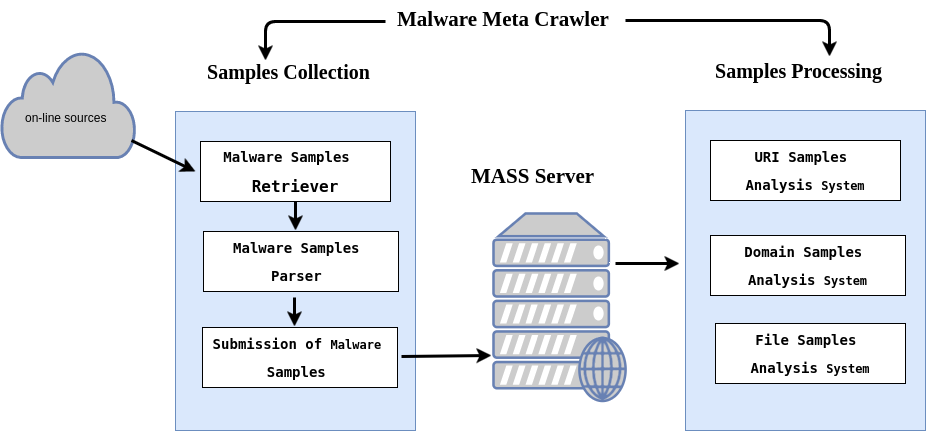
\includegraphics[width=\textwidth,height=.65\textheight]{mass1.png}
     \caption{Generic architecture of the Malware Meta Crawler for MASS System.}
      \label{fig:architecture}
\end{figure}  

\par \textbf{Samples collection:} This subsystem is responsible for the retrieving of malware samples from the different on-line repositories were described the in Section~\ref{sec:sources}. Then the fetched samples are mapped and parsed to the corresponding type (i.e., Domain, URI and File) by this subsystem. Furthermore, 
this subsystem submits the retrieved malware samples  to the MASS server using the MASS API client interface.
\par \textbf{Samples processing:} This subsystem enriches the information of the malware samples retrieved by the sample collection subsystem, also it constructs the relation between the related malware samples. The following are the main modules (i.e., analysis units) of the sample processing subsystem, which automatically receive the new samples submitted to the MASS server:
\begin{itemize}
\item \textbf{URI Samples Analysis Client: }this module is responsible to pull the new malware samples of URI type from the MASS server, in order to find the domain of each URI and submit the relation between them to the MASS server.\newline
\item \textbf{File Samples Analysis Client: } this module identifies the URI of file samples using predefined regular expression, then it tries to download the file from its source and submit it to the MASS server. In addition, it generates the relation between the sample file and origin URI sample.\newline 
\item \textbf{Domain Samples Analysis Client: } this module receives all new domain malware samples, then, it looks up for the domain's IP and connect them by the submitting the IP sample and the relation between them to the MASS server.
\end{itemize}

 

\subsection{Process Flow of System} 

This section presents the process flow of the Malware Meta Crawler system that retrieves the malware samples from different on-line sources to  submit them to the MASS server database. Figure~\ref{fig:processflow} illustrates the internal process of the proposed system. 
 

 \begin{figure}[]
  \centering
     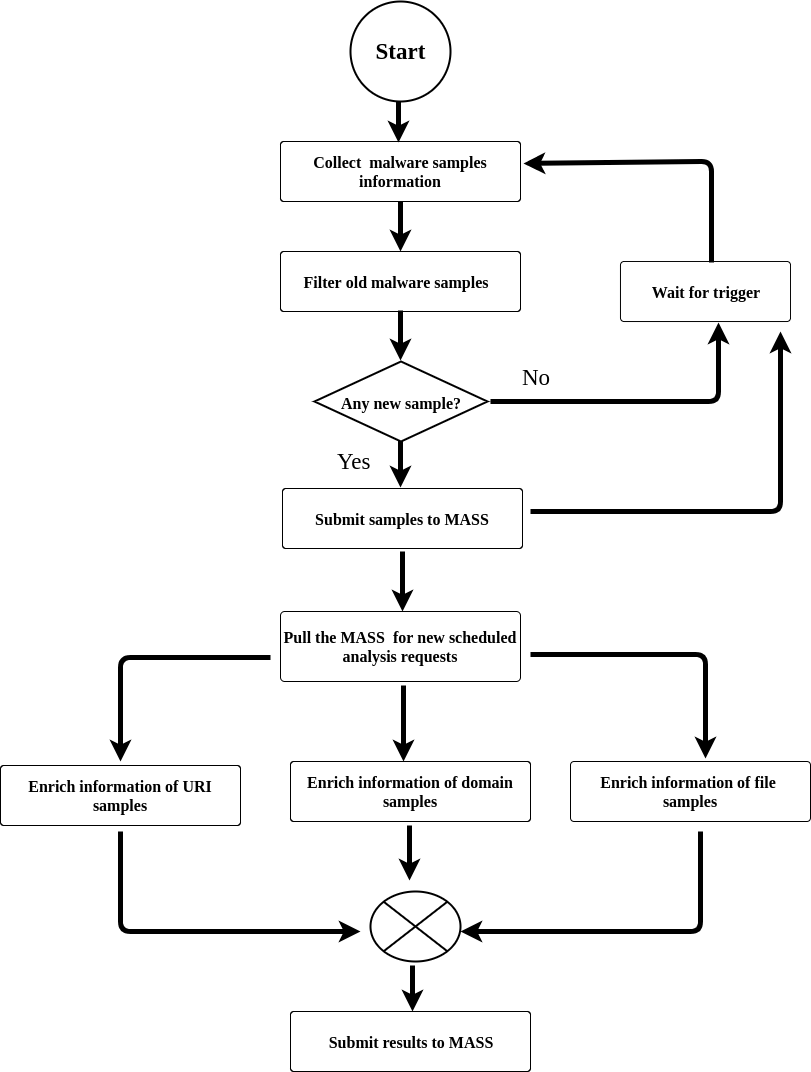
\includegraphics[width=\textwidth, height=\textheight]{mass2.png}
      \caption{Process Flow of Malware Meta Crawler.}
       \label{fig:processflow}
 \end{figure} 


\par  The process begins by collecting the malware samples from the mentioned sources in  Section~\ref{sec:sources}, and these samples include malicious domains and URIs for for infected websites or malware files. The system checks the retrieved samples to filter the old samples  processed and submitted before, and cache information about the  new malware samples in internal storage for later checking. Then the system submits all new malware samples to the MASS server using the offered REST APIs.

\par This process is running again after waiting for the next trigger, which allows to   automate the execution using cron job  that runs the system after certain  period of time or even manual re-execution. This work flow will continue so that the
system can continuously retrieve the new on-line malware samples.

\par On the other hand, MASS schedules new analysis requests for the summited new malware samples by the first part of the system's work flow. Then the three analysis clients pull the scheduled analysis requests that contain the information of new malware samples to enrich their information and generate the relation between the related samples. The following are the analysis processes:     

\begin{itemize}
\item \textbf{Enrich information of URI samples}: this process receives all new URI samples to find the URI's domain and submit the relation between the two samples to MASS.

\item \textbf{Enrich information of domain samples}: this process receives all new domain samples in order to look up for the domain's IP and create a relation between them, received domains includes domains submitted by the system from the on-line repositories and the computed domains from previous process (i.e., domains of URI samples).
\item \textbf{Enrich information of URI file samples}: this process receives all new URI samples to filter the URIs that belong to malware files, using a configured regular expression, then the corresponding file is downloaded and pushed to the MASS server. In addition, this process submits a relation between the downloaded file and its original URI. 

\end{itemize}
\section{Details and Implementation}
\label{sec:sec4}

This section describes the implementation of the various parts of the Malware Meta Crawler for MASS system. The system is implemented in \textbf{Python 3} and the source code is available on GitLab repository\footnote{\url{https://git.cs.uni-bonn.de/lab-mass-ws1617/malware_meta_crawler}}.

\subsection{Collection and Submission of Malware Samples}
This section provides some of main code implementaion of the system's part that retrieves the malware samples and sends them to the MASS server. We use the  \texttt{ConnectionManager} of the \texttt{mass\_api\_client} to fetch content of a given URI as shown in Figure~\ref{sec:conectionManger}.


\inputminted[fontsize=\small, linenos, numbersep=5pt, tabsize=4, frame=lines, breaklines]{python}{task1.py}

\begin{figure}
\caption{Fetching content of a URI Code.}
\label{sec:conectionManger}
\end{figure}

The system parses the content of the different malware samples source based on the content using the following techniques:
 
 \begin{itemize}
 \item \textbf{Parse HTML documents}: we use the \texttt{BeautifulSoup} \footnote{\url{https://www.crummy.com/software/BeautifulSoup/bs4/doc/}} python library 
 to extract the malware data form the retrieved pages.
 
  \item \textbf{Parse XML feed}: some of the malware data is provided in XML format, the  \texttt{xml.dom.minidom} module of Python Standard Library  is used to parse and process the XML data.
  
  \item \textbf{Parse plain text file}: most of the malicious domains are provided in plain text file format which is parsed by our system by simply iterating over the file's lines.
 \end{itemize}
 
 \par The system pushes the fetched malware data to the MASS server using the programing APIs provided by the \texttt{mass\_api\_client}. Figure~\ref{sec:submitSamples} illustrates the different procedures to submit the malware samples to the MASS server.
 
 \inputminted[fontsize=\small, linenos, numbersep=5pt, tabsize=4, frame=lines, breaklines]{python}{task2.py}
 
 \begin{figure}
 \caption{Submission the malware samples to the MASS server.}
 \label{sec:submitSamples}
 \end{figure}
\subsection{Analysis Clients}


MASS offers the feature of scheduling analysis requests for new submitted malware samples, and the analysis systems connect to the MASS server to receive the new samples of the scheduled analysis request. To build a new analysis system the \texttt{mass\_client} \footnote{\url{https://github.com/mass-project/mass_client/tree/master/mass_client}} provides the \texttt{AnalysisClient} base class, we use it in our analysis units that enrich the information of malware sample and create relation between them. 
\par Figure~\ref{sec:analysisClient} shows the code of the \texttt{URISamplesAnalysisInstance} class that processes all URI samples to compute their domain and create the relation between the two samples.

\inputminted[fontsize=\small, linenos, numbersep=5pt, tabsize=4, frame=lines, breaklines]{python}{task3.py}
 
 \begin{figure}
 \caption{URISamplesAnalysisInstance code.}
 \label{sec:analysisClient}
 \end{figure}
\section{System Evaluation}
\label{sec:sec5}
   
 In this section, we present an evaluation of the proposed system. We show how the system perform by measuring  performance metrics including execution time and  memory usage. In addition, the results of the system are evaluated using  statistics of retrieved malware samples and their enriched information in single full execution cycle.
  Also we present the details of the evaluation environment.
 
 \subsection{Environment Setup} 
 
 The evaluations have been conducted on single local machine, Table 1 shows the main hardware and software characteristics of evaluation environment. We evaluate our system by running the our system (including the analysis clients) and the MASS server on the same local machine and observe the performance and statistics metrics. 
 
\begin{center}
   \begin{tabularx}{\textwidth}{ X }
   
   \caption{Test Machine Configurations}\\
   \hline
    \\\large {Hardware configuration} \\\\
     \hline
     CPU \hspace{3.2cm} Intel® Core™ i5-6200U \\
     CPU Speed/Turbo \hspace{1.1cm} 2.30GHz\\
     \#Cores \hspace{2.8cm} 4\\ 
     Memory  \hspace{2.7cm} 16 GB DDR3 \\
     Network \hspace{2.7cm} StudNet Bonn Network  \\
     
     \hline
        \\\large {Software configuration} \\\\
          \hline

               OS Version \hspace{2.3cm} Ubuntu 16.04 LTS \\
               Kernel \hspace{3cm} Linux version 4.4.0-77-generic\\
               Python \hspace{2.9cm} Python 3.5.2\\ 
               MASS version  \hspace{1.9cm} 1.0-alpha1 \\
               \hline 
               
   \end{tabularx}
   
\end{center}
   
 \subsection{Performance Evaluation}
 
 In this section, we present the measurements of the performance metrics (i.e., execution time and memory usage) for the system for full cycle execution and break them down to benchmark the different parts of the system.
 
 \par Table 2 shows the performance results of the two subsystems of the system, we divide  the performance measurements of the malware samples collection subsystem  into two parts. We study the performance of the system regarding the samples retreating from the on-line sources and the submission of samples to the MASS server. on the other hand, we provide the performance qunatites of the three analysis clients that process the malware samples based on their type to enrich their information. All measurements represent the average value of multiple executions. 
 
 \begin{center}
    \begin{tabularx}{\textwidth}{ X }
    
    \caption{Measurements of System Performance }\\
    \hline
     \\\large { Samples collection subsystem} \\\\
      \hline
      \\\hspace{4cm}  Execution time (s)  \hspace{1cm}  Memory usage (MB) \\\\
    
         Samples retrieving \hspace{1.3cm}  6.6  \hspace{3.7cm}  90 \\
      
      Samples submission \hspace{1.2cm}  3,800  \hspace{3.2cm}  111 \\\\
      \hline

 
         \\\large {Samples processing subsystem} \\\\
          \hline
               \\ Analysis client\hspace{1.7cm}  Execution time (s)  \hspace{1cm}  Memory usage (MB) \\\\
             
                  File samples \hspace{2.1 cm} 2.3  \hspace{3.6cm}  35 \\
               
               URI samples  \hspace{2cm}  1.9  \hspace{3.6cm}  33 \\
               
               Domain samples \hspace{1.5cm}  2.1  \hspace{3.6cm}  31 \\
               \hline
                
    \end{tabularx}
    
 \end{center}
 
 
 Results show that process of retrieving malware samples  perform has a good performance profile while the submission of the malware samples process takes more time, which can be improved by parallelizing the push of the samples using multi-threading. On the other hand, the three analysis clients achieves the desired functionalities in a good performance.   

 \subsection{Results Evaluation}
 
  This section provides the details and quantities of the malware samples retrieved by the Malware Meta Crawler system in full execution cycle. Furthermore, an example of the enriched information and relation were generated by the system (i.e., analysis clients) is provided.
  \par Table 3 shows the total number of malware samples that are retrieved by the system within a new execution, it also provides the distribution of samples between the different sources. The results show that the Malware Domain Blocklist gives the largest number of malware samples (malicious domains).
  
  \begin{center}
      \begin{tabularx}{\textwidth}{| X |  X|}
      
      \caption{Number of Malware Samples }\\
     
     
        \hline
        Source \hspace{4cm} &  \# of samples \hspace{4cm} \\ 
        \hline
        Malware Domain Blocklist \hspace{4cm} & 21809  \hspace{4cm} \\ 
        \hline
        Malc0de \hspace{4cm} &  50 \hspace{4cm} \\ 
        \hline
        ZeuS Tracker \hspace{4cm} &  100 \hspace{4cm} \\ 
        \hline
        MalShare \hspace{4cm} &  14 \hspace{4cm} \\ 
        \hline
        Malware URLs \hspace{4cm} &  521 \hspace{4cm} \\ 
        \hline
        URL Query \hspace{4cm} &  20 \hspace{4cm} \\ 
        \hline
        Phish Tank \hspace{4cm} & 520  \hspace{4cm} \\ 
        \hline
        VXVault \hspace{4cm} &  101 \hspace{4cm} \\ 
        \hline
        All sources \hspace{4cm} &  23135 \hspace{4cm} \\ 
        \hline
      \end{tabularx}
          
       \end{center}
       
       \par Figure~\ref{fig:relations} shows an example of the processing results of the three analysis clients (i.e., URI Samples Analysis Client, Domain Samples Analysis Client and File Samples Analysis Client), the relations between the related samples are generated by the three analysis clients.
        \begin{figure}[]
         \centering
            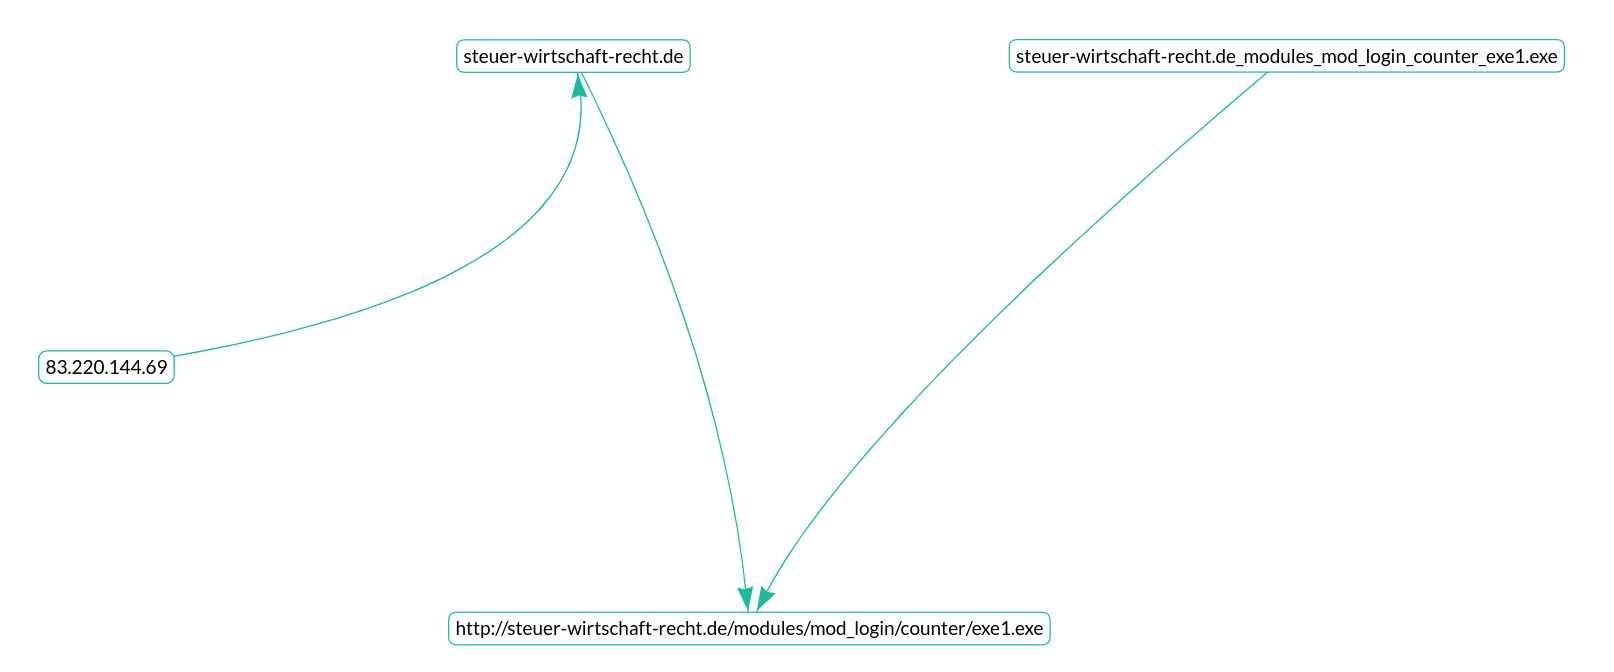
\includegraphics[width=\textwidth]{mass3.png}
             \caption{An example of  relation graph of a malware sample in MASS.}
              \label{fig:relations}
        \end{figure}
       
 \newpage
\section{Conclusion and Future Work}
 \label{sec:sec6}
 
 In this report, we presented a system (i.e., Malware Meta Crawler) that retrieves malware samples from on-line sources and pushes them to the MASS server. The system is divided into two subsystems samples collection and processing. Sample collection subsystem is responsible to retrieve and submit the samples. while  samples processing subsystem is composed of three analysis units (i.e., analysis clients) that receive the submitted malware samples and enrich their information by building the relation between the malware samples. The evaluation of our framework shows that it achieves a good coverage of malware samples with good performance profile.

\par Suggestions for future work include support more malware sources and repositories to increase the coverage of the system, in addition, the performance of samples submission part of the system can be improved by multi-threading integration. 
 
\newpage
\begin{thebibliography}{[MT1]}

%

\bibitem[1]{malware_analysis_def} 
Bayer, Ulrich, et al. "Dynamic analysis of malicious code." Journal in Computer Virology 2.1 (2006): 67-77.

\bibitem[2]{worms} 
Kienzle, Darrell M., and Matthew C. Elder. "Recent worms: a survey and trends." Proceedings of the 2003 ACM workshop on Rapid malcode. ACM, 2003.

\bibitem[3]{symantec} 
Symantec. Internet Security Threat Report, Vol. 21 https://www.symantec.com/content/dam/symantec/docs/reports/istr-21-2016-en.pdf, 2016.

\bibitem[4]{malware_analysis} 
Egele, Manuel, et al. "A survey on automated dynamic malware-analysis techniques and tools." ACM Computing Surveys (CSUR) 44.2 (2012): 6.

\bibitem[5]{mass}
The Malware Analysis and Storage System(MASS). URL https://github.com/mass-project/mass\_server/blob/master/README.md.
Accessed: 2017-04-27.

\bibitem[6]{mass_api}
The MASS API Client. URL https://github.com/mass-project/mass\_api\_client.
Accessed: 2017-04-07.

\bibitem[7]{malware_survey}
Manuel Egele. A survey on automated dynamic
malware analysis techniques and tools. ACM
Computing Surveys, to appear.

\bibitem[8]{bot}
Li, Chao, Wei Jiang, and Xin Zou. "Botnet: Survey and case study." innovative computing, information and control (icicic), 2009 fourth international conference on. IEEE, 2009.

\bibitem[9]{virus}
Spafford, Eugene H. "The Internet Worm Incident Technical Report CSD-TR-933." (1991).


\bibitem[10]{maltrieve}
Maltrieve. URL https://github.com/krmaxwell/maltrieve.
Accessed: 2017-04-25.

\bibitem[11]{ragpicker}
Ragpicker. URL https://code.google.com/archive/p/malware-crawler/.
Accessed: 2017-04-25.

\bibitem[12]{blocklist}
Malware Domains. URL http://www.malwaredomains.com/.
Accessed: 2017-04-20.


\bibitem[13]{malc0de}
Malc0de. URL http://malc0de.com/database/.
Accessed: 2017-04-01.


\bibitem[14]{zeus}
Zeus Tracker. https://zeustracker.abuse.ch/feeds.php.
Accessed: 2017-03-11.


\bibitem[15]{malshare}
Malshare. http://www.malshare.com/index.php.
Accessed: 2017-03-15.

\bibitem[16]{malurls}
Malware URLs. http://malwareurls.joxeankoret.com/.
Accessed: 2017-03-15.

\bibitem[17]{urlQuery}
urlQuery. http://urlquery.net/about.php.
Accessed: 2017-03-05.


\bibitem[18]{phishtank}
Phishtank. http://www.phishtank.com/. 
Accessed: 2017-03-25.


\bibitem[19]{vx}
VX Vault. http://vxvault.net/ViriList.php.
Accessed: 2017-03-25.

\bibitem[20]{python}
Van Rossum, Guido. "Python Programming Language." USENIX Annual Technical Conference. Vol. 41. 2007.
%
\end{thebibliography}

\end{document}